\chapter{Geconjugeerde carbonylverbindingen: Michael en Robinson}\label{ch:b2:conjugate-additions}

De vier ringen van een steroïdhormoon werden eerst ring per ring opgebouwd, en één reeks
reacties werd de standaardmanier om een ring toe te voegen: ze bouwt een volledige zesring, keton
inbegrepen, uit een keton en een klein onverzadigd keton. Dat werkt omdat een carbonylgroep die geconjugeerd is
met een dubbele binding \ce{C=C} haar elektrofiele karakter doorgeeft aan het verre uiteinde van die dubbele binding.
Dit hoofdstuk gaat over dat verre uiteinde: welke nucleofielen het aanvallen, waarom, en wat je ermee kunt bouwen.

\begin{recall}
\Cref{ch:b2:enolates-aldol}: \omterm{def:b2:enolates-aldol:enolate}{enolaten}, de \omterm{def:b2:enolates-aldol:aldol}{aldolcondensatie}. \Cref{ch:b2:frontier-orbitals}:
ladings- en \omterm{def:b2:frontier-orbitals:control}{orbitaalcontrole}, harde en zachte reagentia. \Cref{ch:b2:huckel}: hückelorbitalen en $\pi$-ladingen.
Het deel van jaar~1: grignardreagentia en hydriden, kinetische en thermodynamische controle, geconjugeerde
systemen.
\end{recall}

\section{Twee elektrofiele plaatsen}

\begin{definition}[$\alpha,\beta$-Onverzadigde carbonylverbindingen]\label{def:b2:conjugate-additions:enone}
Een \emph{$\alpha,\beta$-onverzadigde carbonylverbinding}\index{alfa,beta-onverzadigde carbonylverbinding@$\alpha,\beta$-onverzadigde carbonylverbinding}
heeft een dubbele binding \ce{C=C} tussen het $\alpha$-
en het $\beta$-koolstofatoom van een carbonylverbinding, geconjugeerd met de \ce{C=O}: een enon (keton), een enal
(aldehyde), een onverzadigde ester of een onverzadigd \omterm{def:b2:amines:nitrile}{nitril}. De eenvoudigste zijn propenal \ce{CH2=CHCHO} en
but-3-een-2-on \ce{CH2=CHCOCH3} (methylvinylketon).
\end{definition}

\begin{omfigure}
\setchemfig{atom sep=1.9em}
\schemestart
\chemfig{H_2C=CH-CH=O}
\arrow{<->}
\chemfig{H_2C=CH-\chemabove{C}{\scriptstyle +}H-\chemabove{O}{\scriptstyle -}}
\arrow{<->}
\chemfig{\chemabove{C}{\scriptstyle +}H_2-CH=CH-\chemabove{O}{\scriptstyle -}}
\schemestop
\par\medskip

\begin{tikzpicture}
\begin{axis}[ybar, width=0.47\linewidth, height=4.6cm, ymin=-0.6, ymax=0.4,
  xtick={1,2,3,4}, xticklabels={C$\beta$,C$\alpha$,C(O),O}, axis x line=bottom, axis y line=left,
  extra y ticks={0}, extra y tick style={grid=major, grid style={black!50}}, enlarge x limits=0.15,
  tick label style={font=\scriptsize}, ylabel={$\pi$-lading}, label style={font=\small},
  title={\small $\pi$-ladingen van propenal}, bar width=8pt]
\addplot[fill=omDef!50, draw=omDef] table[x=atom, y=q] {figdata/out/bachelor-2-huckel-d.dat};
\end{axis}
\end{tikzpicture}\hfill
\begin{tikzpicture}
\begin{axis}[ybar, width=0.47\linewidth, height=4.6cm, ymin=-0.8, ymax=0.8,
  xtick={1,2,3,4}, xticklabels={C$\beta$,C$\alpha$,C(O),O}, axis x line=bottom, axis y line=left,
  extra y ticks={0}, extra y tick style={grid=major, grid style={black!50}}, enlarge x limits=0.15,
  tick label style={font=\scriptsize}, ylabel={coëfficiënt}, label style={font=\small},
  title={\small LUMO van propenal}, bar width=8pt]
\addplot[fill=omThm!45, draw=omThm] table[x=atom, y=c] {figdata/out/bachelor-2-huckel-d.dat};
\end{axis}
\end{tikzpicture}

{\small Propenal. Boven: zijn drie resonantiestructuren; de laatste twee zetten een positieve lading op het
carbonylkoolstofatoom en op het $\beta$-koolstofatoom. Onder: het hückelmodel van
\cref{ch:b2:frontier-orbitals} ($\alpha_{\ce{O}} = \alpha + \beta$, $\beta_{\ce{CO}} = \beta$; een model).
De grootste positieve lading zit op het carbonylkoolstofatoom (+0.33, tegenover +0.23 op het $\beta$-koolstofatoom); de
grootste LUMO-coëfficiënt zit op het $\beta$-koolstofatoom (0.66, tegenover $-0.58$).}
\end{omfigure}

\begin{proposition}[Twee plaatsen]\label{prop:b2:conjugate-additions:two-sites}
In een $\alpha,\beta$-onverzadigde carbonylverbinding zijn zowel het carbonylkoolstofatoom als het $\beta$-koolstofatoom
elektrofiel. Het carbonylkoolstofatoom draagt de grootste positieve lading; het $\beta$-koolstofatoom draagt de
grootste coëfficiënt in de \omterm{def:b2:frontier-orbitals:frontier}{LUMO}.
\end{proposition}

\begin{proof}[Redenering]
De resonantiestructuren zetten een positieve lading op het carbonylkoolstofatoom en, via de \ce{C=C}, op
het $\beta$-koolstofatoom; het $\alpha$-koolstofatoom is nooit positief. Het hückelmodel van propenal maakt dit
kwantitatief: de som van $2c^2$ over de twee bezette $\pi$-orbitalen geeft de $\pi$-ladingen
(\cref{def:b2:huckel:indices}) $+0.33$ op het carbonylkoolstofatoom, $+0.23$ op het $\beta$-koolstofatoom, $-0.03$
op het $\alpha$-koolstofatoom en $-0.53$ op zuurstof. De \omterm{def:b2:frontier-orbitals:frontier}{LUMO}, de orbitaal die de elektronen van een nucleofiel
ontvangt, is het grootst op het $\beta$-koolstofatoom. De twee plaatsen beantwoorden dus aan de twee soorten controle
van \cref{def:b2:frontier-orbitals:control}.
% figdata: bachelor-2/huckel.py part d
\end{proof}

\section{1,2-Additie of geconjugeerde additie}

\begin{definition}[Wijzen van additie]\label{def:b2:conjugate-additions:addition-modes}
Een nucleofiel dat addeert aan het carbonylkoolstofatoom van een $\alpha,\beta$-onverzadigde carbonylverbinding geeft een
\emph{1,2-additie}\index{1,2-additie} (geteld vanaf het zuurstofatoom): een allylisch alkoxide, en daarna een
alcohol. Een nucleofiel dat addeert aan het $\beta$-koolstofatoom geeft een \emph{geconjugeerde additie}\index{geconjugeerde additie}
(of 1,4-additie): een \omterm{def:b2:enolates-aldol:enolate}{enolaat}, dat op koolstof geprotoneerd wordt en een verzadigde carbonylverbinding
geeft, gesubstitueerd op het $\beta$-koolstofatoom.
\end{definition}

\begin{omfigure}
\setchemfig{atom sep=1.9em}
\schemestart
\chemfig{*6(-=-(=O)---)}
\arrow{->[\ce{CH3Li}][daarna \ce{H2O}]}[,1.4]
\chemfig{*6(-=-(-[:75]CH_3)(-[:-15]OH)---)}
\schemestop
\hspace{2.5em}
\schemestart
\chemfig{*6(-=-(=O)---)}
\arrow{->[\ce{(CH3)2CuLi}][daarna \ce{H2O}]}[,1.6]
\chemfig{*6(-(-CH_3)--(=O)---)}
\schemestop
\par\vspace{6pt}

{\small Cyclohex-2-een-1-on met twee methylnucleofielen. Methyllithium, een \omterm{def:b2:frontier-orbitals:hard-soft}{hard nucleofiel}, addeert aan
het carbonylkoolstofatoom: 1-methylcyclohex-2-een-1-ol (\omterm{def:b2:conjugate-additions:addition-modes}{1,2-additie}). Lithiumdimethylcupraat, een \omterm{def:b2:frontier-orbitals:hard-soft}{zacht nucleofiel},
addeert aan het $\beta$-koolstofatoom: 3-methylcyclohexanon (\omterm{def:b2:conjugate-additions:addition-modes}{geconjugeerde additie}).}
\end{omfigure}

\begin{proposition}[Welke plaats]\label{prop:b2:conjugate-additions:regio}
\omterm{def:b2:frontier-orbitals:hard-soft}{Harde nucleofielen} (organolithiumverbindingen, de meeste grignardreagentia, \ce{LiAlH4}) adderen vooral 1,2, onder \omterm{def:b2:frontier-orbitals:control}{ladingscontrole},
meestal onomkeerbaar. \omterm{def:b2:frontier-orbitals:hard-soft}{Zachte nucleofielen} (\omterm{def:b2:conjugate-additions:cuprate}{organocupraten}, gestabiliseerde \omterm{def:b2:enolates-aldol:enolate}{enolaten}, thiolaten,
aminen) adderen vooral 1,4, onder \omterm{def:b2:frontier-orbitals:control}{orbitaalcontrole}; het geconjugeerde adduct, dat de binding \ce{C=O} behoudt, is
ook het stabielere product.
\end{proposition}

\begin{proof}[Redenering]
Een \omterm{def:b2:frontier-orbitals:hard-soft}{hard nucleofiel}, klein en geladen, gaat vooral via ladingen in wisselwerking: het gaat naar het meest positieve
centrum, het carbonylkoolstofatoom (\cref{prop:b2:conjugate-additions:two-sites}); zijn additie is snel en
keert niet terug, dus het 1,2-product, dat sneller gevormd wordt, blijft (kinetische controle). Een \omterm{def:b2:frontier-orbitals:hard-soft}{zacht nucleofiel},
groot en polariseerbaar, met een hoge \omterm{def:b2:frontier-orbitals:frontier}{HOMO}, gaat vooral via de \omterm{def:b2:frontier-orbitals:frontier}{grensorbitalen} in wisselwerking: het gaat naar waar
de \omterm{def:b2:frontier-orbitals:frontier}{LUMO} het grootst is, het $\beta$-koolstofatoom. Het 1,4-product behoudt een $\pi$-binding van \ce{C=O}, sterker dan de
$\pi$-binding van \ce{C=C} die het 1,2-product behoudt; wanneer de addities omkeerbaar zijn (cyanide, aminen,
gestabiliseerde \omterm{def:b2:enolates-aldol:enolate}{enolaten}, alkoxiden), schuift het evenwicht daarom naar het geconjugeerde adduct, zelfs wanneer het
1,2-adduct eerst gevormd werd (thermodynamische controle).
\end{proof}

\begin{method}[De wijze van additie voorspellen]\label{met:b2:conjugate-additions:predict-mode}
\begin{enumerate}
  \item Deel het nucleofiel in: hard (\ce{RLi}, \ce{RMgX}, \ce{LiAlH4}, \ce{NaBH4} met een aldehyde)
        of zacht (\ce{R2CuLi}, een 1,3-dicarbonylenolaat, \ce{RS-}, \ce{R2NH}, cyanide bij evenwicht).
  \item Controleer de omkeerbaarheid: een onomkeerbare harde additie geeft het 1,2-product; een omkeerbare
        geeft, met de tijd, het 1,4-product.
  \item Controleer de hindering: een gesubstitueerd $\beta$-koolstofatoom vertraagt de 1,4-additie; een aldehyde, minder gehinderd
        en reactiever aan zijn carbonylgroep dan een keton, begunstigt 1,2.
  \item Schrijf het \omterm{def:b2:enolates-aldol:enolate}{enolaat} op dat de 1,4-additie vormt: het kan geprotoneerd worden, of weggevangen door een
        elektrofiel.
\end{enumerate}
\end{method}

\section{Michaeladdities}

\begin{definition}[Michaeladditie]\label{def:b2:conjugate-additions:michael}
Een \emph{michaeladditie}\index{michaeladditie} is de \omterm{def:b2:conjugate-additions:addition-modes}{geconjugeerde additie} van een gestabiliseerd carbanion,
meestal een \omterm{def:b2:enolates-aldol:enolate}{enolaat}, aan een $\alpha,\beta$-onverzadigde carbonylverbinding of een vergelijkbaar elektronenarm
alkeen. Het nucleofiel is de \emph{michaeldonor}\index{michaeldonor} (een 1,3-dicarbonylverbinding, een
nitroalkaan, een cyaanester); de onverzadigde verbinding is de \emph{michaelacceptor}\index{michaelacceptor}
(een enon, een enal, een onverzadigde ester, een onverzadigd \omterm{def:b2:amines:nitrile}{nitril} of een onverzadigde nitroverbinding).
\end{definition}

\begin{omfigure}
\setchemfig{atom sep=1.8em}
\schemestart
\chemfig{CH_2(-[:30]COOEt)(-[:-30]COOEt)}
\arrow{<=>[\ce{EtO-}][$-$ \ce{EtOH}]}[,1.3]
\chemfig{\chemabove{C}{\scriptstyle -}H(-[:30]COOEt)(-[:-30]COOEt)}
\+
\chemfig{H_2C=CH-C(=[2]O)-CH_3}
\schemestop

\medskip
\setchemfig{atom sep=1.6em}
\schemestart
\arrow{->[additie]}[,0.95]
\chemfig{CH(-[:150]EtOOC)(-[:210]EtOOC)-CH_2-CH=C(-[2]\chemabove{O}{\scriptstyle -})-CH_3}
\arrow{->[\ce{EtOH}][$-$ \ce{EtO-}]}[,1.1]
\chemfig{CH(-[:150]EtOOC)(-[:210]EtOOC)-CH_2-CH_2-C(=[2]O)-CH_3}
\schemestop
\par\vspace{6pt}

{\small De \omterm{def:b2:conjugate-additions:michael}{michaeladditie} van diethylpropaandioaat aan but-3-een-2-on. Ethoxide vormt het gestabiliseerde
\omterm{def:b2:enolates-aldol:enolate}{enolaat}; dat addeert aan het $\beta$-koolstofatoom; het gevormde \omterm{def:b2:enolates-aldol:enolate}{enolaat} neemt een proton op van ethanol, wat
ethoxide terugvormt. Het product, diethyl-(3-oxobutyl)propaandioaat, is een
1,5-dicarbonylverbinding.}
\end{omfigure}

\begin{proposition}[Mechanisme van Michael]\label{prop:b2:conjugate-additions:michael}
Een \omterm{def:b2:conjugate-additions:michael}{michaeladditie} verloopt in drie stappen (deprotonering van de donor, \omterm{def:b2:conjugate-additions:addition-modes}{geconjugeerde additie}, protonering van
het nieuwe \omterm{def:b2:enolates-aldol:enolate}{enolaat}), en de base wordt in de laatste stap teruggevormd: een katalytische hoeveelheid volstaat.
\end{proposition}

\begin{proof}[Redenering]
Het $\alpha$-waterstofatoom van de donor, tussen twee carbonylgroepen, is zuur: $\mathrm pK_a$ ongeveer 13 voor
diethylpropaandioaat, 10.7 voor ethyl-3-oxobutanoaat. Ethoxide (ethanol, 15.9) haalt het grotendeels weg, wat
ruim voldoende is. Het gestabiliseerde, zachte \omterm{def:b2:enolates-aldol:enolate}{enolaat} addeert 1,4
(\cref{prop:b2:conjugate-additions:regio}). Het gevormde \omterm{def:b2:enolates-aldol:enolate}{enolaat} is een sterkere base dan het \omterm{def:b2:enolates-aldol:enolate}{enolaat} van de donor
(het is gestabiliseerd door één carbonylgroep, niet twee), dus het neemt een proton op van het oplosmiddel, wat
één ethoxide teruggeeft voor het verbruikte. De totale reactie vormt een $\sigma$-binding \ce{C-C} uit een
$\pi$-binding \ce{C=C}: ze is gunstig, en met een gestabiliseerde donor keert het adduct niet terug.
% ledger: pka:ethanol, pka:diethylmalonate, pka:acetoacetate
\end{proof}

Een michaeladduct met een keton aan de kant van de donor en een aan de kant van de acceptor is een
1,5-dicarbonylverbinding: de twee carbonylgroepen liggen vijf koolstofatomen uit elkaar, beide carbonylkoolstofatomen meegeteld. Dat patroon is het
kenmerk van een \omterm{def:b2:conjugate-additions:michael}{michaeladditie}, zoals de $\beta$-hydroxycarbonylverbinding dat van de \omterm{def:b2:enolates-aldol:aldol}{aldolreactie} was
(\cref{met:b2:enolates-aldol:aldol-recognition}).

\section{Organocupraten}

\begin{definition}[Organocupraten]\label{def:b2:conjugate-additions:cuprate}
Een \emph{organocupraat}\index{organocupraat} \ce{R2CuLi} is een koper(I)verbinding met twee organische
groepen, gemaakt uit twee equivalenten van een organolithiumverbinding en één van een koper(I)halogenide:
\begin{equation*}
\ce{2 CH3Li + CuI -> (CH3)2CuLi + LiI}.
\end{equation*}
\end{definition}

\omterm{def:b2:conjugate-additions:cuprate}{Organocupraten} (ook gilmanreagentia genoemd) worden bereid en gebruikt in ether bij lage temperatuur onder
inert gas, zoals de organolithiumverbindingen waarvan ze afgeleid zijn. Koper is minder elektropositief dan lithium of
magnesium, dus de binding \ce{Cu-C} is meer covalent en het koolstofatoom minder geladen: de methylgroep van een
cupraat is een \omterm{def:b2:frontier-orbitals:hard-soft}{zacht nucleofiel}. Daaruit volgen drie toepassingen.

\begin{itemize}
  \item \emph{\omterm{def:b2:conjugate-additions:addition-modes}{Geconjugeerde additie}} van een alkyl- of arylgroep aan een enon, wat grignardreagentia en
        organolithiumverbindingen niet zuiver doen; slechts een van de twee groepen \ce{R} wordt overgedragen.
  \item \emph{Wegvangen}: het \omterm{def:b2:enolates-aldol:enolate}{enolaat} dat de \omterm{def:b2:conjugate-additions:addition-modes}{geconjugeerde additie} vormt, kan op zijn $\alpha$-koolstofatoom
        gealkyleerd worden, zodat in één bewerking twee nieuwe bindingen \ce{C-C} ontstaan.
  \item \emph{Substitutie} van halogeniden: $\mathrm{R_2CuLi + R'Br \to R{-}R' + RCu + LiBr}$, een koppeling die een
        organolithiumverbinding zou bederven door eliminatie of uitwisseling.
\end{itemize}

\section{De robinsonannulatie}

\begin{definition}[Annulatie]\label{def:b2:conjugate-additions:robinson}
Een \emph{annulatie}\index{annulatie} bouwt een nieuwe ring aan een bestaand molecuul. De \emph{robinsonannulatie}
\index{robinsonannulatie} bouwt een cyclohex-2-een-1-on op: een \omterm{def:b2:conjugate-additions:michael}{michaeladditie} van het \omterm{def:b2:enolates-aldol:enolate}{enolaat} van een keton
aan een $\alpha,\beta$-onverzadigd keton (meestal but-3-een-2-on), gevolgd door een
intramoleculaire \omterm{def:b2:enolates-aldol:aldol}{aldolcondensatie} van het gevormde 1,5-diketon.
\end{definition}

\begin{omfigure}
\setchemfig{atom sep=1.8em}
\schemestart
\chemfig{[:30]*6(-(=O)-(-CH_3)-(=O)---)}
\+
\chemfig{=[:30]-[:-30](=[:-90]O)-[:30]}
\arrow{->[base][Michael]}[,1.2]
\chemfig{[:30]*6(-(=O)-(-[:40]CH_3)(-[:-30]-[:30]-[:-30](=[:-90]O)-[:30])-(=O)---)}
\schemestop

\medskip
\schemestart
\arrow{->[base][aldol]}[,1.1]
\chemfig{[:-30]*6(---(-[:-60]OH)*6(--(=O)---)-(-[:105]CH_3)-(=O)-)}
\arrow{->[verhitten][$-$ \ce{H2O}]}[,1.1]
\chemfig{[:-30]*6(---*6(=-(=O)---)-(-[:105]CH_3)-(=O)-)}
\schemestop
\par\vspace{6pt}

{\small De \omterm{def:b2:conjugate-additions:robinson}{robinsonannulatie} die het Wieland--Miescher-keton maakt. Het \omterm{def:b2:enolates-aldol:enolate}{enolaat} van
2-methylcyclohexaan-1,3-dion addeert aan but-3-een-2-on (Michael): een triketon. Het \omterm{def:b2:enolates-aldol:enolate}{enolaat} van het
methylketon in de zijketen valt een carbonylgroep van de ring aan (intramoleculaire \omterm{def:b2:enolates-aldol:aldol}{aldolreactie}) en sluit een zesring;
dehydratatie geeft het geconjugeerde enon. De angulaire methylgroep zit op het koolstofatoom dat de twee
ringen delen, het enige stereocentrum.}
\end{omfigure}

\begin{proposition}[Robinsonannulatie]\label{prop:b2:conjugate-additions:robinson}
Een keton met een $\alpha$-waterstofatoom en but-3-een-2-on geven in base een cyclohex-2-een-1-on in drie
stappen: \omterm{def:b2:conjugate-additions:michael}{michaeladditie}, intramoleculaire \omterm{def:b2:enolates-aldol:aldol}{aldoladditie} die een zesring vormt, en dehydratatie.
De nieuwe ring bevat het vroegere $\alpha$-koolstofatoom van het keton en zijn carbonylkoolstofatoom, en de vier
koolstofatomen van but-3-een-2-on.
\end{proposition}

\begin{proof}
Volg de atomen in de figuur. Het enolaatkoolstofatoom van het keton (noem het C$_a$) bindt aan het $\beta$-koolstofatoom
van but-3-een-2-on: de keten C$_a$--\ce{CH2}--\ce{CH2}--\ce{C(=O)}--\ce{CH3} hangt aan C$_a$, en
C$_a$ is nog gebonden aan het carbonylkoolstofatoom C$_k$ van het keton. In base vormt het methylketon van de keten
zijn \omterm{def:b2:enolates-aldol:enolate}{enolaat} aan de eindstandige \ce{CH3}, dat C$_k$ aanvalt. De gesloten ring telt C$_k$, C$_a$,
de twee \ce{CH2}, het carbonylkoolstofatoom van de zijketen en het vroegere methylkoolstofatoom: zes atomen, de spanningsvrije
ringgrootte, en daarom leidt dit \omterm{def:b2:enolates-aldol:enolate}{enolaat}, van de mogelijke \omterm{def:b2:enolates-aldol:enolate}{enolaten}, tot een stabiel product (een
aanval door het \omterm{def:b2:enolates-aldol:enolate}{enolaat} van de inwendige \ce{CH2} van de keten zou een vierring sluiten). Het \omterm{def:b2:enolates-aldol:aldol}{aldol} heeft zijn
\ce{OH} op C$_k$, $\beta$ ten opzichte van de carbonylgroep van de keten; dehydratatie zet de \ce{C=C} tussen C$_k$ en het
vroegere methylkoolstofatoom, geconjugeerd met de carbonylgroep: een cyclohex-2-een-1-on.
\end{proof}

\begin{method}[Disconnectie van een cyclohexenon]\label{met:b2:conjugate-additions:robinson-disconnection}
\begin{enumerate}
  \item Zoek een cyclohex-2-een-1-on in het doelmolecuul; nummer zijn carbonylkoolstofatoom C1, de dubbele binding
        C2=C3, en de ring verder tot C6.
  \item Maak de dehydratatie ongedaan: een \ce{OH} op C3, een \ce{C-H} op C2.
  \item Maak de \omterm{def:b2:enolates-aldol:aldol}{aldolreactie} ongedaan: knip C2--C3 door. C3 wordt een carbonylgroep van een keton, C2 een methylgroep van een
        methylketon: een 1,5-diketon.
  \item Maak de \omterm{def:b2:conjugate-additions:michael}{michaeladditie} ongedaan: knip de binding door tussen C4 (het $\alpha$-koolstofatoom van het keton op C3) en
        C5. De donor is dat keton; de acceptor is het enon C5=C6--C1(=O)--C2, dat
        but-3-een-2-on is wanneer C5, C6 en C2 alleen waterstofatomen dragen.
\end{enumerate}
\end{method}

\begin{history}[De annulatie, 1935]
\begin{minipage}[t]{0.18\linewidth}
\vspace{0pt}
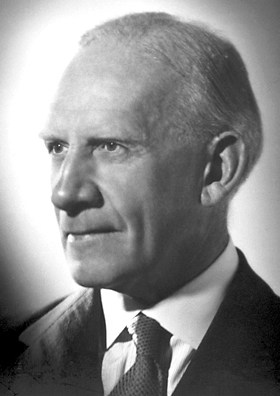
\includegraphics[width=\linewidth]{images/book3/robinson.jpg}
\end{minipage}\hfill
\begin{minipage}[t]{0.78\linewidth}
\vspace{0pt}
Robert Robinson en William Rapson publiceerden de ringvormende reeks in 1935, in werk dat gericht was op de
synthese van steroïden. Robinsons belangrijkste verwezenlijkingen waren de structuren en syntheses van alkaloïden,
waarvoor hij in 1947 de Nobelprijs voor de Scheikunde kreeg. In 1950 maakten Peter Wieland en Karl Miescher
het bicyclische diketon van het probleem van dit hoofdstuk, dat een gebruikelijk uitgangspunt werd voor syntheses van steroïden en
terpenen. (Portret: onbekende auteur, publiek domein; Wikimedia Commons.)
\end{minipage}
\end{history}

\begin{safety}{\ghs[5mm]{GHS02}\,\ghs[5mm]{GHS05}\,\ghs[5mm]{GHS06}\,\ghs[5mm]{GHS07}\,\ghs[5mm]{GHS08}\,\ghs[5mm]{GHS09}}
But-3-een-2-on is ontvlambaar, zeer giftig, corrosief en schadelijk voor het aquatisch milieu, en een sterk traanverwekkend middel; het wordt alleen
in een zuurkast gehanteerd. Cyclohex-2-een-1-on is ontvlambaar en giftig. Organolithiumverbindingen, grignardreagentia en
cupraten reageren heftig met water en worden onder inert gas gehanteerd.
% ledger: ghs:MVK, ghs:cyclohexenone, ghs:MeMgBr
\end{safety}

\section{Oefeningen}

\begin{exercise}[$\star$]\label{exo:b2:conjugate-additions:1}
Voorspel 1,2- of 1,4-additie aan cyclohex-2-een-1-on voor: \ce{CH3MgBr}; \ce{(CH3)2CuLi};
\ce{C6H5SH} met een beetje base; \ce{LiAlH4}.
\end{exercise}

\begin{exercise}[$\star$]\label{exo:b2:conjugate-additions:2}
Deel in als \omterm{def:b2:conjugate-additions:michael}{michaeldonor} of \omterm{def:b2:conjugate-additions:michael}{michaelacceptor}: pentaan-2,4-dion, propeennitril \ce{CH2=CHCN},
nitromethaan, methylpropenoaat, diethylpropaandioaat, but-3-een-2-on.
\end{exercise}

\begin{exercise}[$\star$]\label{exo:b2:conjugate-additions:3}
Schrijf de bereiding op van lithiumdibutylcupraat uit 1-broombutaan, lithium en koper(I)jodide.
\end{exercise}

\begin{exercise}[$\star$]\label{exo:b2:conjugate-additions:4}
Geef het product van diethylpropaandioaat met but-3-een-2-on en een katalytische hoeveelheid
natriumethoxide, en daarna het product na hydrolyse en verhitten.
\end{exercise}

\begin{exercise}[$\star\star$]\label{exo:b2:conjugate-additions:5}
Stel een bereiding voor van 3-methylcyclohexanon uit cyclohex-2-een-1-on, en leg uit waarom
methylmagnesiumbromide een slechte keuze zou zijn.
\end{exercise}

\begin{exercise}[$\star\star$]\label{exo:b2:conjugate-additions:6}
Ethaanthiol addeert aan but-3-een-2-on met een spoor triethylamine. Schrijf het mechanisme op en zeg waarom het
thiolaat 1,4 addeert.
\end{exercise}

\begin{exercise}[$\star\star$]\label{exo:b2:conjugate-additions:7}
Cyanide geeft met cyclohex-2-een-1-on bij lage temperatuur en korte tijden het cyaanhydrine; bij hogere
temperatuur en langere tijden 3-oxocyclohexaan-1-carbonitril. Verklaar met kinetische en thermodynamische
controle.
\end{exercise}

\begin{exercise}[$\star\star$]\label{exo:b2:conjugate-additions:8}
Geef het product van de \omterm{def:b2:conjugate-additions:robinson}{robinsonannulatie} van 2-methylcyclohexaan-1,3-dion met but-3-een-2-on, en daarna dat
van cyclohexanon met but-3-een-2-on.
\end{exercise}

\begin{exercise}[$\star\star$]\label{exo:b2:conjugate-additions:9}
Maak een disconnectie van heptaan-2,6-dion in een \omterm{def:b2:conjugate-additions:michael}{michaeldonor} en een \omterm{def:b2:conjugate-additions:michael}{michaelacceptor}, en stel omstandigheden voor.
\end{exercise}

\begin{exercise}[$\star\star\star$]\label{exo:b2:conjugate-additions:10}
Een eenvoudige \omterm{def:b2:enolates-aldol:aldol}{aldoladditie} wordt in base gemakkelijk omgekeerd; het michaeladduct van diethylpropaandioaat en
but-3-een-2-on niet. Verklaar met de gevormde en verbroken bindingen en met de zuurgraad van het product.
\end{exercise}

\begin{exercise}[$\star\star\star$]\label{exo:b2:conjugate-additions:11}
Diethylpropaandioaat geeft met twee equivalenten methylpropenoaat en een katalytische base een product
zonder resterende \ce{C-H} tussen zijn twee estergroepen. Teken het en leg uit.
\end{exercise}

\begin{exercise}[$\star\star\star$]\label{exo:b2:conjugate-additions:12}
2-Methylcyclohexanon en but-3-een-2-on kunnen in een \omterm{def:b2:conjugate-additions:robinson}{robinsonannulatie} via elk van beide \omterm{def:b2:enolates-aldol:enolate}{enolaten} reageren.
Teken beide producten en zeg welke omstandigheden het product begunstigen met de methylgroep op het koolstofatoom
van de ringverbinding.
\end{exercise}

\section{Probleem: het Wieland--Miescher-keton}

\begin{problem}[{Weekendprobleem --- de zure donor, het michaeladduct, de intramoleculaire aldolreactie en
haar dehydratatie, het stereocentrum en de massabalans van een bereiding}]
\label{pb:b2:conjugate-additions:1}
Bereiding (gegevens voor de oefening): \qty{10.0}{g} 2-methylcyclohexaan-1,3-dion reageert met een lichte overmaat
but-3-een-2-on en een katalytische base (\omterm{def:b2:conjugate-additions:michael}{michaeladditie}); het triketon wordt daarna gecycliseerd met een
\omterm{def:b2:amines:class}{secundair amine} en een zuur (\omterm{def:b2:enolates-aldol:aldol}{aldolreactie}, dehydratatie). Totaal rendement: 70~\%. Het moedermolecuul cyclohexaan-1,3-dion
heeft $\mathrm pK_a = 5.3$ in water. Molaire massa's (\unit{g/mol}): C 12.011, H 1.008, O 15.999.
% ledger: pka:cyclohexanedione, aw:C, aw:H, aw:O, ghs:methylcyclohexanedione, ghs:MVK

\medskip
\noindent\textbf{Deel I --- De donor.}
\begin{enumerate}
  \item Teken 2-methylcyclohexaan-1,3-dion en markeer zijn zuurste waterstofatoom.
  \item Waarom is dat waterstofatoom zoveel zuurder dan de $\alpha$-waterstofatomen van cyclohexanon?
  \item Teken de drie resonantiestructuren van zijn \omterm{def:b2:enolates-aldol:enolate}{enolaat}.
  \item Is hydroxide of ethoxide sterk genoeg om dit \omterm{def:b2:enolates-aldol:enolate}{enolaat} volledig te vormen? Gebruik de $\mathrm pK_a$.
  \item Schrijf het \omterm{def:b2:enolates-aldol:tautomerism}{enol} van het dion op waarbij C2 betrokken is, en zeg waarom de methylgroep op C2 dat
        niet verhindert.
  \item Is dit \omterm{def:b2:enolates-aldol:enolate}{enolaat} hard of zacht? Welke plaats van but-3-een-2-on zal het aanvallen?
\end{enumerate}

\medskip
\noindent\textbf{Deel II --- Het michaeladduct.}
\begin{enumerate}[resume]
  \item Schrijf de \omterm{def:b2:conjugate-additions:michael}{michaeladditie} op en geef de naam van het gevormde triketon.
  \item Waarom is er maar een katalytische hoeveelheid base nodig?
  \item Waarom vormt de nieuwe binding zich op C2 van het dion en niet op zijn zuurstofatoom?
  \item Hoeveel quaternaire koolstofatomen heeft het triketon?
  \item Wijs de 1,5-dicarbonylrelatie in het triketon aan.
  \item Waarom wordt een lichte overmaat but-3-een-2-on gebruikt, en waarom maar een lichte?
\end{enumerate}

\medskip
\noindent\textbf{Deel III --- De ringsluiting.}
\begin{enumerate}[resume]
  \item Som de koolstofatomen van het triketon op die $\alpha$-waterstofatomen dragen.
  \item Welk \omterm{def:b2:enolates-aldol:enolate}{enolaat}, dat welke carbonylgroep aanvalt, sluit een zesring?
  \item Welke andere ringsluitingen zou men kunnen proberen, en waarom geven ze het product niet?
  \item Schrijf het gevormde \omterm{def:b2:enolates-aldol:aldol}{aldol} op en de dehydratatie die volgt.
  \item Waarom verloopt de dehydratatie gemakkelijk?
  \item Geef de functionele groepen van het Wieland--Miescher-keton.
\end{enumerate}

\medskip
\noindent\textbf{Deel IV --- Stereochemie en massabalans.}
\begin{enumerate}[resume]
  \item Welk koolstofatoom van het product is een stereocentrum?
  \item Is het product van deze bereiding optisch actief? Leg uit.
  \item Bereken de molaire massa's van het dion, van but-3-een-2-on en van het product
        \ce{C11H14O2}.
  \item Schrijf de totale vergelijking op en controleer ze met de formules.
  \item Bereken de gebruikte hoeveelheid dion.
  \item Geef de massa Wieland--Miescher-keton die verkregen wordt bij een totaal rendement van 70~\%.
\end{enumerate}
\end{problem}
